\documentclass[extra]{gji}
%~ \documentclass[extra, referee]{gji}

\usepackage[utf8]{inputenc}
\usepackage{timet}
\usepackage{amsmath}
\usepackage{graphicx}
%~ \usepackage{todonotes} % to make annotations on margins
\usepackage[disable]{todonotes} % to disable annotations on margins

\usepackage{url}
\usepackage[pdftex,colorlinks=true]{hyperref}
\hypersetup{
    allcolors=blue,
}


\begin{document}

\title[Variable Density Tesseroids]{
    Variable Density Tesseroids: Gravity fields calculation in spherical coordinates using variable densities in depth
}
\author[S.R. Soler, L. Uieda and M.E. Gimenez]{
    Santiado R. Soler$^{1,2}$, Leonardo Uieda$^3$ and Mario E. Gimenez$^{1,2}$ \\
    $^1$CONICET, Argentina. e-mail: santiago.r.soler@gmail.com\\
    $^2$Instituto Geofísico Sismológico Volponi, Universidad Nacional de San Juan, Argentina\\
    $^3$Universidade do Estado do Rio de Janeiro, Rio de Janeiro, Brazil
    }


\maketitle

\begin{summary}
Summary of this paper 
\end{summary}

\begin{keywords}
Satellite gravity??, Numerical modelling, Structure of the Earth, Gravity anomalies and Earth structure, Numerical approximations and analysis, spatial analysis??
\end{keywords}


\section{Introduction}

Lithosphere's density variation with depth has been studied for almost a century. 
On the first years \citet{Athy1930} obtained a decreasing exponential relation between both quantities by studying shale samples, while in the following decades other density functions have been proposed for different rock types \citep[e.g.,][]{Maxant1980, Rao1986, Rao1993, Rao1994}.
Furthermore, the density variation with depth has been taken into account in forward and inversion gravity models, mostly applied to grabens and basins \citep{Cordell1973, Rao1986, Cowie1990, Rao1993, Rao1994, Zhang2001, Welford2010}.

These forward gravity models have been developed for two or three dimensional bodies in cartesian coordinates that properly fit local scales applications.
Nevertheless, the latest satellite missions have provided us gravity measurements with global coverage, which allows geologists and geophysics to perform modelling and interpretation on regional scales.
This raises the importance of building forward models that reproduce the gravity anomalies for such scales.

The main issue that should be overcome is taking into account the curvature of the Earth, thus the forward model must be defined in spherical coordinates.
A common way to achieve this is to discretize the Earth in spherical prisms known as tesseroids, which are defined by pairs of latitude, longitude and radius boundaries (see Figure \ref{fig:tesseroid-uieda}).
Calculating the gravity fields generated by an arbitrary tesseroid on any external point involves the resolution of volume integrals that are generally approximated by numerical computations.
The literature offers two approaches: one involves Taylor series expansion \citep{Heck2007, Grombein2013} while the other makes use of Gauss-Legendre Quadrature (GLQ) \citep{Asgharzadeh2007, Uieda2016, Uieda2017}.
The later consists in approximating the integral by a weighted sum of the effect of point masses located at scaled nodes of the Legendre polynomials.

\begin{figure}
\centering
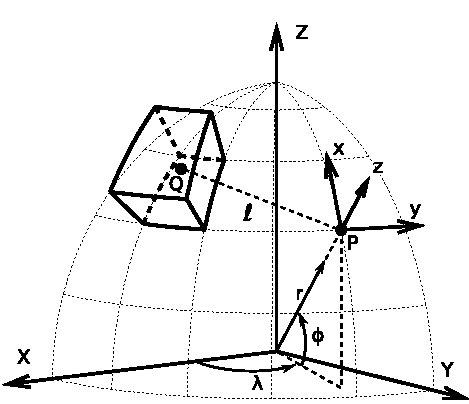
\includegraphics[width=0.9\linewidth]{figures/tesseroid-uieda.pdf}
\caption{
A spherical prism, also known as  Tesseroid, in a geocentric spherical coordinate system, with a computation point $P$ and its local north oriented Cartesian coordinate system. Picture made by \citet{Uieda2015}.
}
\label{fig:tesseroid-uieda}
\end{figure}

\citet{Uieda2016} developed a forward gravity model based on tesseroids with homogeneous densities using the GLQ approximation method.
It has been originally implemented through command line programs written in C programming language.
However, it has been ultimately ported to Python and included in the open-source library Fatiando a Terra \citep{Uieda2013} for geophysical modelling and inversion.

In order to develop a forward model that computes the gravity field generated by any tesseroid with arbitrary variable density, the Taylor series expansion is not well suited, because it would need to derive the series expansion terms for each density function.
On the other hand, the GLQ allows us to calculate them for any density function without any other information but the function itself.

\citet{Ku1977} documented that the GLQ becomes less accurate when the computation point is closer to the tesseroid or for smaller GLQ order. 
Although the model developed by \citet{Uieda2016} uses a second order GLQ, it ensures the accuracy implementing a modified version of the adaptive discretization of \citet{Li2011}.
It consist in splitting the tesseroid into smaller ones when a certain distance-size ratio is lower than a predefined value ($D$) that controls the accuracy of the computation. 
\citet{Uieda2016} have also objectively obtained standard values of $D$ for gravity potential, gradients and tensor components comparing the fields generated by a spherical shell, which constitutes a special case of the volume integrals that has analytical solution \citep{LaFehr1991, Mikuska2006, Grombein2013}\todo{citar mas??}.

We have enhanced the later implementation with a new forward gravity model that allows us to compute the gravity fields generated by any tesseroid with an arbitrary density function on any external point.
It's based on the GLQ approximation, makes use of the modified distance-size discretization algorithm and is written in Python and Cython languages, obtaining an easy to use library that runs precompiled code for the more time consuming functions.

In order to ensure the accuracy of the numerical approximation, we have conducted similar tests as the one performed by \citet{Uieda2016} by comparing the results of the numerical model with the analytical solutions for a spherical shell with linear, exponential and discontinuous density.
Furthermore we had to derive the analytical expressions for these density functions.

This new forward gravity model makes use of some previously existing classes and functions from Fatiando a Terra, what saved us time and allowed us to focus on the new enhancements.
Furthermore, we have the intention to include it into a future release of the Fatiando a Terra library in order to make its distribution and maintenance easier.

In the following sections we will describe how the new algorithm works, its theoretical background and obtain the distance-size ratio values needed to get a good accuracy in the computation.

%%%%%%%%%%%%%%%%%%%%%%%%%%%%%%%%%%%%%%%%%%%%%%%%%%%%%%%%%%%%%%%%%%%%%%%%%%%%%%

\section{Theory}

The spherical prisms known as tesseroids are mass elements defined in a geocentric spherical coordinate system bounded by a pair of parallels, a pair of  meridians, and two concentric spherical surfaces.
We define an external computation point $P(r, \phi, \lambda)$ where the gravity fields generated by the tesseroid are going to be calculated with respect to the local north oriented Cartesian coordinate system located at $P$.
In the special case of homogeneous density, the gravity potential, its gradient and the Marussi tensor components can be calculated through the integrals obtained by \citet{Grombein2013} \citep[see also][]{Uieda2016}.

In our case, we will assume that the tesseroid has an arbitrary variable density in depth, i.e. only depends on the radius spherical coordinate.
Thus, the integrals for the gravity fields are slightly modified:

\begin{equation}
    V(r,\phi,\lambda) = G
    \int\limits_{\lambda_1}^{\lambda_2}
    \int\limits_{\phi_1}^{\phi_2}
    \int\limits_{r_1}^{r_2}
    \frac{\rho(r')}{\ell} \kappa \,  dr' d\phi' d\lambda',
\label{eq:tesseroid-pot}
\end{equation}
\begin{equation}
    g_{\alpha}(r,\phi,\lambda) = G
    \int\limits_{\lambda_1}^{\lambda_2}
    \int\limits_{\phi_1}^{\phi_2}
    \int\limits_{r_1}^{r_2}
    \rho(r') \frac{\Delta_\alpha}{\ell^3}
    \kappa \, dr' d\phi' d\lambda',
\label{eq:tesseroid-grav}
\end{equation}
\begin{equation}
    g_{\alpha\beta}(r,\phi,\lambda) = G
    \int\limits_{\lambda_1}^{\lambda_2}
    \int\limits_{\phi_1}^{\phi_2}
    \int\limits_{r_1}^{r_2}
    \rho(r') I_{\alpha\beta} \, \kappa \, dr' d\phi' d\lambda' ,
    \label{eq:tesseroid-tensor}
\end{equation}

\noindent where

\begin{equation}
    I_{\alpha\beta} =
    \left(
        \frac{3\Delta_{\alpha} \Delta_{\beta}}{\ell^5} -
        \frac{\delta_{\alpha\beta}}{\ell^3}
    \right) ,
    \label{eq:tesseroid-tensor-kernel}
\end{equation}

\noindent $\alpha, \beta \in \{x, y, z\}$,
$\rho(r')$ is the density function that depends on the radius coordinate,
$\delta_{\alpha\beta}$ is Kronecker's delta,
$G = 6.674\times10^{-11}\, \text{m$^3$kg$^{-1}$s$^{-1}$}$ is the gravitational constant and

\begin{equation}
    \Delta_x = r'[\cos\phi\sin\phi' - \sin\phi\cos\phi'
               \cos(\lambda' - \lambda)],
\end{equation}
\begin{equation}
    \Delta_y = r' \cos \phi' \sin(\lambda' - \lambda),
\end{equation}
\begin{equation}
    \Delta_z = r' \cos \psi - r,
\end{equation}
\begin{equation}
    \kappa = {r'}^2 \cos \phi',
\end{equation}
\begin{equation}
    \ell = \sqrt{{r'}^2 + r^2 - 2 r' r \cos \psi},
\label{eq:ell}
\end{equation}
\begin{equation}
    \cos\psi = \sin\phi\sin\phi' + \cos\phi\cos\phi'
                 \cos(\lambda' - \lambda).
\label{eq:cospsi}
\end{equation}


According to \citet[p.~390]{Hildebrand1987}, we can approximate any integral in the interval $[-1, 1]$ using a $N$th order GLQ, i.e. by a weighted sum of the integration kernel evaluated on the roots of the $N$th Legendre polynomial:

\begin{equation}
    \int\limits_{-1}^1 f(x) dx \approx \frac{b-a}{2} \sum_{i=1}^N W_i f(x_i),
\end{equation}

\noindent where $x_i$ are the roots of the $N$th Legendre polynomial $P_N(x)$ and $W_i$ are the weights of each term:

\begin{equation}
    W_i = \frac{2}{(1-x_i^2)[P_N^\prime(x_i)]^2},
\end{equation}

\begin{equation}
    P_N(x_i) = 0, \quad \forall i = {1,\dots,N}.
\end{equation}

In case of an integration defined on a arbitrary interval, e.g. $[a,b]$, we can scale the nodes and perform a similar approximation:

\begin{equation}
    \int\limits_a^b f(x) dx \approx \frac{b-a}{2} \sum_{i=1}^N W_i f(x_i^s),
\label{eq:glq-scaled}
\end{equation}

\noindent where $x_i^s$ is the scaled $x_i$ root in the $[a,b]$ interval, also called nodes of the quadrature:

\begin{equation}
    x_i^s = \frac{b-a}{2} x_i + \frac{b+a}{2}.
\end{equation}

For example, if we use a second order GLQ, the roots of the $P_2(x)$ Legendre polynomial and its corresponding weights are $x_i = \pm 0.577350269$ and $W_i = 1$.

Our intention is to use GLQ to approximate the volume integrals from equations \ref{eq:tesseroid-pot}-\ref{eq:tesseroid-tensor}. 
When tesseroids have variable densities, we can write the integral kernels as the product of a certain function $g$ and the density function:

\begin{equation}
    f(r', \phi', \lambda') = \rho(r') g(r', \phi', \lambda'),
\end{equation}

\noindent and then apply the quadrature to every integral corresponding to each spherical coordinate, obtaining a similar expression to the one shown by \citet{Asgharzadeh2007} and \citet{Uieda2016}:

\iftwocol{
\begin{equation}
    \begin{split}
        \iiint\limits_\Omega \rho(r') g(r', \phi', \lambda') 
        d\Omega \approx& \\
        A 
        \sum\limits_{i=1}^{N^r}
        \sum\limits_{j=1}^{N^\phi}
        \sum\limits_{k=1}^{N^\lambda}
        & W_i^r W_j^\phi W_k^\lambda \rho(r_i) g(r_i, \phi_j, \lambda_k),
    \end{split}
\label{eq:glq-var-dens}
\end{equation}
}{
\begin{equation}
    \iiint\limits_\Omega \rho(r') g(r', \phi', \lambda') d\Omega \approx
    A 
    \sum\limits_{i=1}^{N^r}
    \sum\limits_{j=1}^{N^\phi}
    \sum\limits_{k=1}^{N^\lambda}
    W_i^r W_j^\phi W_k^\lambda \rho(r_i) g(r_i, \phi_j, \lambda_k),
\label{eq:glq-var-dens}
\end{equation}
}

\noindent where

\begin{equation}
    A = 
    \frac{(\lambda_2 - \lambda_1)(\phi_2 - \phi_1)(r_2 - r_1)}{8}.
\end{equation}

From equation \ref{eq:glq-var-dens} we can observe that the GLQ approximates the gravity fields of a tesseroid with variable density as the ones generated by point masses located at the nodes of the Legendre polynomials.
Furthermore, the information of the density function is summarised as the values it assumes on those nodes.
Although this may sound discouraging, we intent to prove otherwise and show that this method, along with a well fitted discretization algorithm, approximates the gravity fields with good accuracy and precision.\todo{no se si poner esta ultima oracion}

%%%%%%%%%%%%%%%%%%%%%%%%%%%%%%%%%%%%%%%%%%%%%%%%%%%%%%%%%%%%%%%%%%%%%%%%%%%%%%

\subsection{Analytical Solutions for Spherical Shell}

The integrals that define the gravity fields in equations \ref{eq:tesseroid-pot}-\ref{eq:tesseroid-tensor} have analytical solutions for the exceptional case of a spherical shell with homogeneous density \citep{Mikuska2006,Grombein2013}.
In order to test the accuracy of their approximations, \citet{Uieda2016} and \citet{Grombein2013} compared their numerical models (tesseroids with homogeneous density) with these analytical solutions.

In case of variable density tesseroids, the comparison must obviously be made with a variable density spherical shell, whose analytical solution will depend on the chosen density function.
Because the literature has not offered it yet, we had to develop it ourselves. \todo{ no se si ponerlo asi}

Lets consider a spherical shell with inner and outer radii $R_1$ and $R_2$, respectivetly, whose density depends on the radius spherical coordinate (Figure \ref{fig:spherical-shell}).
The gravity potential generated by the shell on an arbitrary external point $Q(0,0,r)$, located along the $z$ axe at a distance $r$ from the origin, can be written as follows:

\begin{figure}
\centering
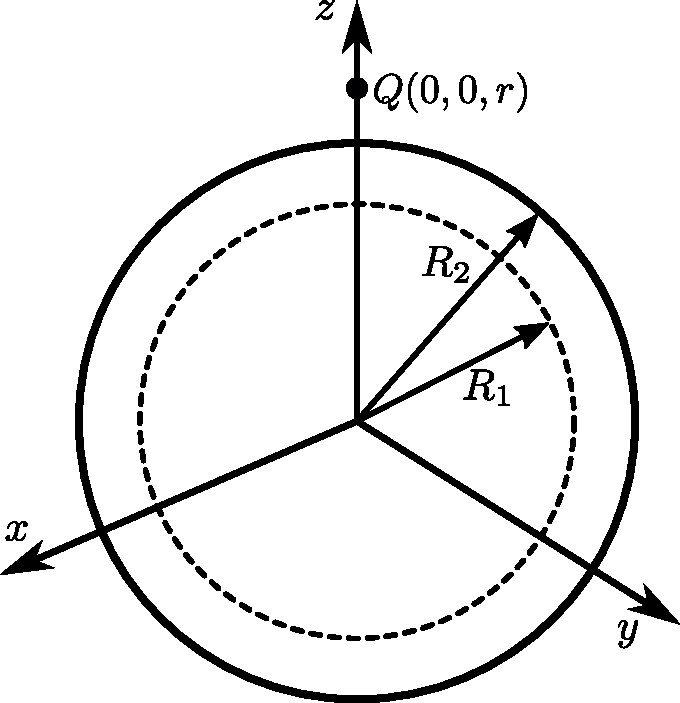
\includegraphics[width=0.7\linewidth]{figures/spherical-shell.pdf}
\caption{
Spherical shell with inner and outer radii $R_1$ and $R_2$, respectively.
The computation point $Q$ is located in the $z$ axe at a distance $r$ from the centre of the shell.
For practical purposes we will assume that $Q$ is outside the outer radii, i.e. $r > R_2$.
}
\label{fig:spherical-shell}
\end{figure}

\begin{equation}
    V_\text{sh}(r) = G 
    \int\limits_0^{2\pi}
    \int\limits_{-\frac{\pi}{2}}^\frac{\pi}{2}
    \int\limits_{R_1}^{R_2}
    \frac{\rho(r')}{\ell} {r'}^2 \cos\phi' \, 
    dr' d\phi' d\lambda',
\end{equation}

\noindent where $\ell$ is defined in equation \ref{eq:ell}.
The computation point $Q$ is located at latitude $\phi=90^\circ$, so $\ell$ and $\cos\psi$ (defined in equation \ref{eq:cospsi}) get simplified:

\begin{equation}
    \cos\psi = \sin\phi', \quad
    \ell = \sqrt{r'^2 - 2 r r' \sin\phi' + r^2}.
\end{equation}

Due to the rotational symmetry along the $z$ axe, the integration in $\lambda'$ is straightforward:

\begin{equation}
    V_\text{sh}(r) = 2\pi G 
    \int\limits_{-\frac{\pi}{2}}^\frac{\pi}{2}
    \int\limits_{R_1}^{R_2}
    \frac{\rho(r') {r'}^2 \cos\phi'}{\sqrt{r'^2 - 2 r r' \sin\phi' + r^2}}
    \, dr' d\phi',
\end{equation}

\noindent and the integration in $\phi'$ can be performed independently of the density function.
Using \citet{sagemath} we obtain the following expression:

\iftwocol{
\begin{equation}
    \begin{split}
        V_\text{sh}(r) = 2\pi G
        \int\limits_{R_1}^{R_2}
        \Big[ & \sqrt{r^2 + r'^2 + 2rr'} - \\
        & \sqrt{r^2 + r'^2 - 2rr'}
        \Big] \frac{r'\rho(r')}{r} \, dr'.
    \end{split}
\label{eq:shell-pot-sqrts}
\end{equation}
}{
\begin{equation}
    V_\text{sh}(r) = 2\pi G
    \int\limits_{R_1}^{R_2}
    \Big[ \sqrt{r^2 + r'^2 + 2rr'}  -
    \sqrt{r^2 + r'^2 - 2rr'} 
    \Big] \frac{r'\rho(r')}{r} \, dr'.
\label{eq:shell-pot-sqrts}
\end{equation}
}

For our purposes we can assume that the computation point $Q$ is outside the outer radii, i.e. $r>R_2$ ($R_2 \geq r'$), and simplify the square roots in equation \ref{eq:shell-pot-sqrts}:

\begin{equation}
    \sqrt{r^2 + r'^2 + 2rr'} = |r + r'| = r + r',
\end{equation}
\begin{equation}
    \sqrt{r^2 + r'^2 - 2rr'} = |r - r'| = r - r',
\end{equation}

\noindent what leads to the following expression of the potential of the spherical shell:

\begin{equation}
    V_\text{sh}(r) = \frac{4\pi G}{r}
    \int\limits_{R_1}^{R_2} {r'}^2 \rho(r') \, dr'.
\label{eq:shell-pot}
\end{equation}

The equation \ref{eq:shell-pot} allows to easily obtain the exact gravity field generated by a spherical shell with a variable density in depth on any outside point located in the $z$ axe.
Due to the rotational symmetry along any axe that passes through the centre of the shell, the integral in equation \ref{eq:shell-pot} reproduces the gravity potential field on any outside point at distance $r$ from the its centre.

The gradient and the Marussi tensor derived from potentials that depends solely on $r$ has only a few non zero components: the vertical component of the gradient ($g_z$) and the diagonal components of the tensor ($g_{xx}$, $g_{yy}$, $g_{zz}$).
They can be easily obtained as \citet{Grombein2013} does, even for any density function $\rho(r')$ of our choice:

\begin{equation}
    g_z = \frac{V_\text{sh}(r)}{r},
\end{equation}
\begin{equation}
    g_{xx} = g_{yy} = -\frac{V_\text{sh}(r)}{r^2}, \quad
    g_{zz} = \frac{2V_\text{sh}(r)}{r^2}.
\end{equation}

For practical purposes we are going to obtain the gravity potential for three different functions from the perspective of their variation in $r'$: a linear and an exponential density function.


\subsubsection{Linear Density}

If the density of the spherical shell is a linear function on the radius coordinate, i.e.:

\begin{equation}
    \rho(r') = ar' + b,
\end{equation}

\noindent then the gravity potential generated on any computation point at distance $r$ from its centre can be obtained from the following expression:

\begin{equation}
    V_\text{sh}^\text{lin}(r) = \pi G \left[ 
    a \frac{R_2^4 - R_1^4}{r} +
    b \,\frac{4}{3} \frac{R_2^3 - R_1^3}{r} \right].
    \label{eq:shell-pot-linear}
\end{equation}

The second term on equation \ref{eq:shell-pot-linear} reproduces the potential generated by a spherical shell with homogeneous density $\rho = b$ \citep{Mikuska2006,Grombein2013}.
So it can be read as the combination of a spherical shell with the later homogeneous density and the same shell with variable density $\rho(r') = ar'$.


\subsubsection{Exponential Density}

If, on the other hand, the spherical shell has an exponential density in the radius coordinate,

\begin{equation}
    \rho(r') = Ae^{-(r' - \Delta h)/b},
\end{equation}

\noindent the potential can be written as follows:

\iftwocol{
\begin{equation}
    \begin{split}
        V_\text{sh}^\text{exp}(r) = \frac{4\pi G}{r} 
        Ab \, e^\frac{\Delta h}{b}
        \Big[
        & (R_1^2 + 2R_1 b + 2b^2)e^{-\frac{R_1}{b}} - \\
        & (R_2^2 + 2R_2 b + 2b^2)e^{-\frac{R_2}{b}}
        \Big].
    \end{split}
\label{eq:shell-pot-exp}
\end{equation}
}{
\begin{equation}
    V_\text{sh}^\text{exp}(r) = \frac{4\pi G}{r} 
    Ab \, e^\frac{\Delta h}{b}
    \Big[
    & (R_1^2 + 2R_1 b + 2b^2)e^{-\frac{R_1}{b}} - \\
    & (R_2^2 + 2R_2 b + 2b^2)e^{-\frac{R_2}{b}}
    \Big].
\label{eq:shell-pot-exp}
\end{equation}
}

%%%%%%%%%%%%%%%%%%%%%%%%%%%%%%%%%%%%%%%%%%%%%%%%%%%%%%%%%%%%%%%%%%%%%%%%%%%%%%%

\section{Implementation}

We have developed a Python library that computes the gravity fields generated by any Tesseroid with variable density in depth through the GLQ to numerically approximate the volume integrals.
It's freely available under the BSD 3-clause open-source library and can be downloaded from the following repository: \todo{agregar repo, vale la pena poner el link?}

Although it's a Python library, the core functions of the computation are written in Cython, a superset of Python language that allows to generate efficient C code through the Cython compiler.
This produces a precompiled library whose functions can be called from regular Python code, what allowed us to make it compatible with the preexisting open-source library Fatiando a Terra \citep{Uieda2013}.

Its usage is very similar to the code for homogeneous tesseroid already in Fatiando a Terra (version 0.5):

\begin{enumerate}
\renewcommand{\theenumi}{(\arabic{enumi})}
    \item Define a single tesseroid (or a tesseroid mesh) with the Fatiando a Terra classes.
    \item Add a predefined Python density function to the tesseroid (or each tesseroid in the mesh).
    \item Calculate the desired gravity field (potential, gradient or tensor component) in any set of computation points with our new functions.
\end{enumerate}

The existing code in Fatiando a Terra (v.~0.5) for homogeneous tesseroid is optimised through the Numba compiler.
Due to difficulties when passing a Python function as argument of precompiled Numba methods, we have decided to rewrite them in Cython language, keeping the homogeneous tesseroid calculation and adding the new variable density code.

From equation \ref{eq:glq-var-dens} we saw that the GLQ approximates the volume integrals as the gravitational effect of $N_\lambda N_\phi N_r$ point masses, where $N_i$ are the orders of the quadrature for the integral on each coordinate, with $i \in \{ \lambda, \phi, r \}$.
If we set the GLQ orders to fixed values, it's easy to conclude that the nearer the computation point is to the tesseroid, the accuracy of the approximation is reduced and the point masses effect becomes more noticeable than the tesseroid we want to approximate.
A more complete analysis of this conclusion can be found in \citet{Ku1977, Li2011, Uieda2016}.

Instead of increasing the GLQ orders to improve the accuracy, what leads to a more time consuming computation, adaptive discretization algorithms have been applied in previous works \citep{Li2011, Uieda2016}.
They essentially consist in dividing the tesseroid based on a ratio between the distance from its geometric centre to the computation point and its dimensions.

In order to make the computation more efficient, we use only second order GLQ for each integration while we ensure the accuracy of the method through the application of the modified adaptive discretization algorithm developed by \citet{Uieda2016}.
The modifications made by \citet{Uieda2016} to the original adaptive discretization method \citep{Li2011} can be summed up in:
(1) a faster calculation of the distance from the computation point to the tesseroid and 
(2) the application of a stack based algorithm that speeds up the computation and gives more control over the recursion step.

More specifically, \citet{Uieda2016} redefined the dimensions of an arbitrary tesseroid: $L_\lambda$, $L_\phi$ and $L_r$. The former ones are the arc-distances measured along its top surface while $L_r$ is the difference between the radii of the top and bottom surfaces.

The adaptive discretization algorithm starts by checking that the following inequality is satisfied:

\begin{equation}
    \frac{d}{L_i} \geq D,
\label{eq:distance-size-ratio}
\end{equation}

\noindent where $i \in \{\lambda, \phi, r\}$, $d$ is the distance between the geometric centre of the tesseroid and the computation point, and $D$ is a predefined value called distance-size ratio.
If the inequality \ref{eq:distance-size-ratio} is not held for any spherical coordinate, then the tesseroid must be divided by half in that direction.
A more complete description of the modified adaptive discretization algorithm can be found in \citet{Uieda2016}.
On the contrary, if the inequality is satisfied, the algorithm computes the desired gravity field using the GLQ approximation.

In summary, the distance-size ratio $D$ determines indirectly how many times the tesseroids will be divided, and therefore regulates both the accuracy of the algorithm and its computation time.
In this way the modified version of the adaptive discretization algorithm efficiently improves its accuracy and gives the user more control over the computation: it allows to stop the division of the tesseroids when their dimensions are lower than a certain value (e.g. less than 10 cm), in which case it does not modifies significantly the desired gravitational field.

On the other hand, the value assigned to the distance-size ratio $D$ cannot be easily related to the error of the approximation, thus the choice of the value of $D$ to get an acceptable accuracy is a matter of study.

In order to overcome this, \citet{Uieda2016} compared the numerical computation with the analytical solution for a spherical shell with homogeneous density.
We have performed similar tests, but now with variable density spherical shell.
From the infinite density functions that can be proposed, we have chosen three characteristic ones: a linear, an exponential and a discontinuous function.


%%%%%%%%%%%%%%%%%%%%%%%%%%%%%%%%%%%%%%%%%%%%%%%%%%%%%%%%%%%%%%%%%%%%%%%%%%%%%%%

\section{Determination of distance-size ratio}

In order to test the new variable density tesseroid code and estimate the error of the approximation, we have compared the numerical model with the analytical solutions for a spherical shell with variable density for three special cases: a linear, an exponential and a discontinuous density function.
The first one constitutes the simplest variation, while the second one represents the fastest varying function. The later one tries to emulate a contact between two different media (e.g. crust and mantle interface).

This error estimations are also useful in the determination of the minimum value for the distance-size ratio $D$ such the difference between the numerical model and the analytical solutions are below an acceptable threshold.

We approximated the spherical shell by a mesh of $30^\circ \times 30^\circ$ tesseroids and calculated the gravity potential, the vertical component of the gradient ($g_z$) and the diagonal components of the Marussi tensor ($g_{xx}$, $g_{yy}$, $g_{zz}$) on four different grids: (1) a grid located at the pole, (2) another one on the Equator, (3) one located at satellite height and (4) a big grid of $30^\circ \times 30^\circ$.
More information about this grids can be found in the Table \ref{tab:grids}.

We computed the three gravity fields  on every point of these four grids for different values of $D$, ranging from 0.5 to 10 with a step of 0.5.
Then we calculated the maximum difference between these results and the value of the analytical solution at the same height.

Because the gravity fields generated by a tesseroid are approximated by the effect of point masses, the numerical results may vary between computation points at same height but at different latitude or longitude.
That's why we choose for comparison the maximum difference between the results on every point of the grid and the analytical solution.

Finally, we set the acceptable value of $D$ if the corresponding error of the numerical approximation is lower than 0.1\%.

\begin{table}
\caption{
    Description of the synthetic grids on which the comparison of the numerical model against the analytical solutions for a spherical shell was done. This collection of grids tries to include every possible scenario on which the numerical model can present a different behaviour depending on the size of the grid, its location or its height over the Earth surface. Every grid consists in a set of 10$\times$10 points.
}
\label{tab:grids}
\begin{tabular}{lcccc}
    Grid & Size & Lat. extension & Lon. extension & Height \\ \hline
    Pole & $1^\circ \times 1^\circ$ & $89^\circ - 90^\circ$ & $0^\circ - 1^\circ$ & 2km \\
    Equator & $1^\circ \times 1^\circ$ & $0^\circ - 1^\circ$ & $0^\circ - 1^\circ$ & 2km \\
    Satellite & $1^\circ \times 1^\circ$ & $89^\circ - 90^\circ$ & $0^\circ - 1^\circ$ & 260km \\
    Big Grid & $30^\circ \times 30^\circ$ & $60^\circ - 90^\circ$ & $0^\circ - 30^\circ$ & 2km \\
\end{tabular}
\end{table}


\subsection{Linear Density}

In first place, we proposed a spherical shell with linear density in such way that it has a density of 2670~kg/m$^3$ on the surface of the Earth, and 3300~kg/m$^3$ at 35 km of depth:

\begin{equation}
    \rho(r') = ar' + c,
    \label{eq:density-linear}
\end{equation}
\noindent with 
\begin{equation}
    a = -\frac{3300\text{kg/m$^3$} - 2670\text{kg/m$^3$}}{35000\text{m}},
\end{equation}
\begin{equation}
    c = \frac{3300\text{kg/m$^3$} - 
        2670\text{kg/m$^3$}}{35000\text{m}} R + 
        2670\text{kg/m$^3$},
\end{equation}

\noindent where $R$ = 6378.137 km is the mean Earth radius.

Then we computed the difference between the numerical model with its corresponding analytical solution (equation \ref{eq:density-linear}) for a thick and a thin spherical shell of 1km and 35km of thickness, respectively.

In Figures \ref{fig:D-linear-thin} and \ref{fig:D-linear-thick} we can see the results for the potential, the vertical component of the gradient $g_z$ and the $g_{zz}$ component of the Marussi tensor.
Because the other two diagonal components of the tensor show similar results as the ones obtained for the $g_{zz}$, we exclude them from the figure, although they can be found in the repository. \todo{chequear}

For the linear density case, we can observe that the calculation of the potential and the $g_z$ component of its gradient needs a value of $D=1$ and $D=2$, respectively, in order to ensure an accuracy of 0.1\%.
On the other hand, the $g_{zz}$ computations show a noticeable difference between the thin and the thick shell: the first one needs a value of $D$ equal to 8 while the later only a $D$ of 3.5.
We will keep the more conservative result of $D$ equal to 8 in case of computing the Marussi tensor components in case of a linear density tesseroid.

\begin{figure}
\centering
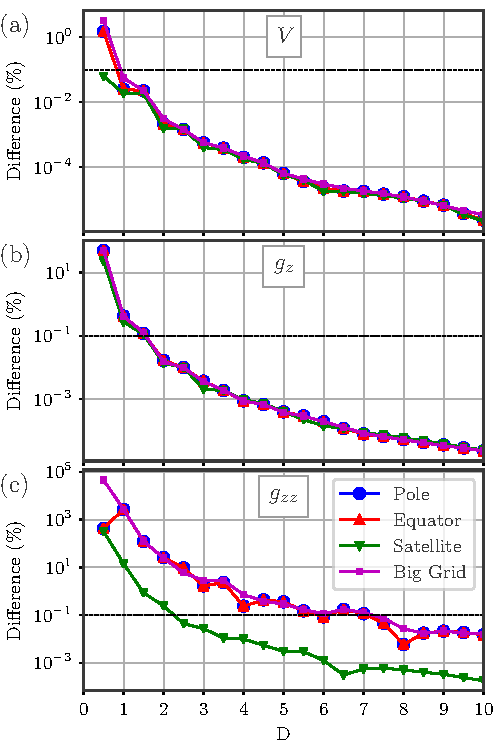
\includegraphics[width=0.9\linewidth]{figures/Dlinear-thin-differences.pdf}
\caption{
    Differences between the gravity fields generated by the numerical model and the analytical solution for a thin spherical shell of 1km of thickness with the linear density defined on equation \ref{eq:density-linear}. The computations were performed on the four grids described in Table \ref{tab:grids} and for different values of the distance-size ratio $D$. If the difference is less than 0.1\%, we consider that the model has achieved an acceptable accuracy for the corresponding value of $D$.
}
\label{fig:D-linear-thin}
\end{figure}

\begin{figure}
\centering
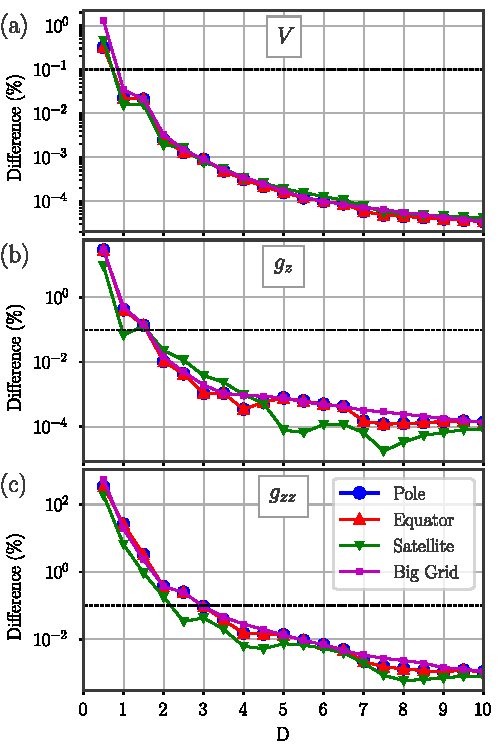
\includegraphics[width=0.9\linewidth]{figures/Dlinear-thick-differences.pdf}
\caption{
    Differences between the gravity fields generated by the numerical model and the analytical solution for a thick spherical shell of 35km of thickness with the linear density defined on equation \ref{eq:density-linear}. The computations were performed on the four grids described in Table \ref{tab:grids} and for different values of the distance-size ratio $D$. If the difference is less than 0.1\%, we consider that the model has achieved an acceptable accuracy for the corresponding value of $D$.
}
\label{fig:D-linear-thick}
\end{figure}


\subsection{Exponential Density}

To test the model in case of an exponential density we proposed the following function:

\begin{equation}
    \rho(r') = A e^{-(r' - R)/b}
\label{eq:density-exp}
\end{equation}

\noindent where $A$ = 1kg/m$^3$ and $b$ = 1000km.
We have performed this test also with a thin and a thick shell of 1 km and 35 km, respectively, whose results can be seen in Figures \ref{fig:D-exp-thin} and \ref{fig:D-exp-thick}.
Once again, the results for $g_{xx}$ and $g_{yy}$ are very similar to the ones obtained for $g_{zz}$, so we exclude them, although, they can be found in the repository.

In the same way we analysed the linear density results, we can summarise that the thin spherical shell presents the more conservative values of the distance-size ratio: $D=1$ for the gravity potential, $D=2$ for its gradient components and $D=8$ for the Marussi tensor components.

Surprisingly both the linear and the exponential density tesseroid models needs the same values of distance-size ratio $D$ in order to assure a good accuracy.

\begin{figure}
\centering
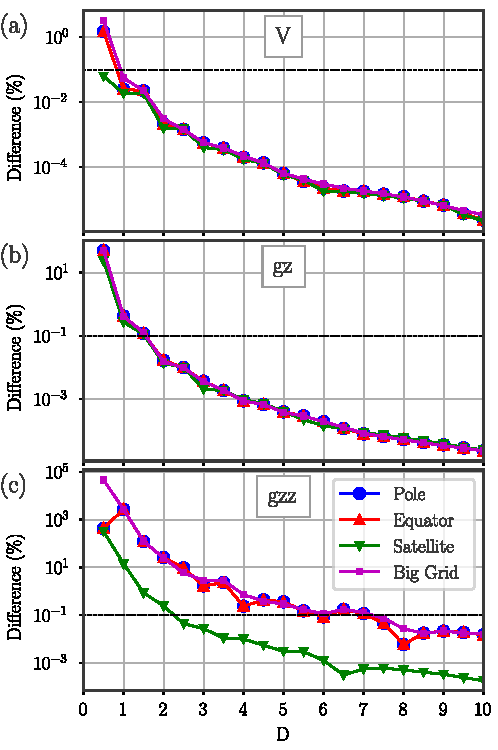
\includegraphics[width=0.9\linewidth]{figures/Dexp-shifted-thin-differences.pdf}
\caption{
    Differences between the gravity fields generated by the numerical model and the analytical solution for a thin spherical shell of 1km of thickness with the exponential density defined on equation \ref{eq:density-exp}. The computations were performed on the four grids described in Table \ref{tab:grids} and for different values of the distance-size ratio $D$. If the difference is less than 0.1\%, we consider that the model has achieved an acceptable accuracy for the corresponding value of $D$.
}
\label{fig:D-exp-thin}
\end{figure}

\begin{figure}
\centering
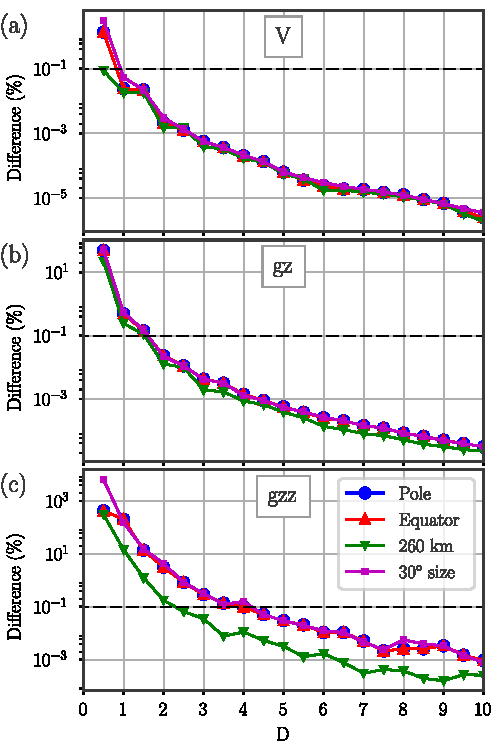
\includegraphics[width=0.9\linewidth]{figures/Dexp-shifted-thick-differences.pdf}
\caption{
    Differences between the gravity fields generated by the numerical model and the analytical solution for a thick spherical shell of 35km of thickness with the exponential density defined on equation \ref{eq:density-exp}. The computations were performed on the four grids described in Table \ref{tab:grids} and for different values of the distance-size ratio $D$. If the difference is less than 0.1\%, we consider that the model has achieved an acceptable accuracy for the corresponding value of $D$.
}
\label{fig:D-exp-thick}
\end{figure}

Because the constant $b$ controls the variation of the density function, we wanted to test how does the accuracy of the method behaves at different values of $b$.
In order to do this we proposed a set of density functions, each one with a different value of $b$ and normalised in such way that they reaches a density of 2900 kg/m$^{3}$ at the bottom of the spherical shell.
We computed the difference between the Marussi tensor component $g_{zz}$ generated by the numerical model on the big grid of 30$^\circ\times$30$^\circ$ (see Table \ref{tab:grids}) and the respective analytical solution.
These differences were calculated for each proposed density function and for the same set of values of $D$ we have been using on the previous tests, obtaining one curve for each value of $b$.

This tests were performed using both the thin and the thick spherical shell.
On Figures \ref{fig:D-exp-power-thin}a and \ref{fig:D-exp-power-thick}a we can see the density functions used to perform these tests for each spherical shell model, respectively, and their results can be seen in \ref{fig:D-exp-power-thin}b and \ref{fig:D-exp-power-thick}b.
Taking into account that lower values of $b$ implies a more varying function, we can see that for extremely varying functions the numerical model does not perform well: for $b$=100m the difference is almost 100\% in the thin shell case, and the same happens with $b$=10km in the thick shell case.

On both cases, the model performs under the acceptable threshold for values of $b$ greater than the thickness of the shell, in other words, when the absolute value of the exponent in equation \ref{eq:density-exp} is lower than one.
Although this sets a limitation to the model, the maximum acceptable variation is very far from real density distributions inside the Earth.
For example, if we take into account a tesseroid with 35km of thickness, a density of 2670kg/m$^3$ on its top surface and $b=35$km, then the density at its bottom will be approximately of 7000kg/m$^3$, very far from the values we can find at such depths.

\begin{figure}
\centering
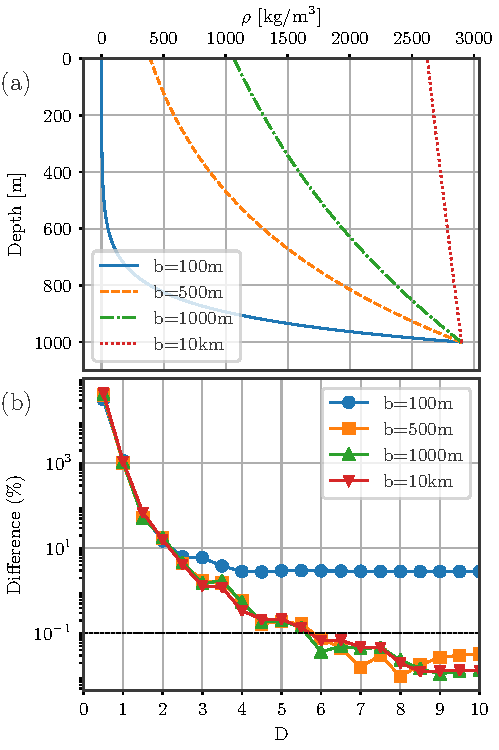
\includegraphics[width=0.9\linewidth]{figures/Dexp-power-differences-thin.pdf}
\caption{
    Results of the accuracy tests for different exponential density functions in case of a thin spherical shell (1km of thickness).
    (a) Density functions used in the tests, each one with a different value of $b$ and normalised in such way that they reaches a density of 2900kg/m$^{3}$ at the bottom of the shell.
    (b) Differences between the Marussi tensor component $g_{zz}$ generated by the numerical model and the analytical solution for each density function. Each computation was performed on the big grid described in Table \ref{tab:grids}, for different values of the distance-size ratio $D$. If the difference is less than 0.1\%, we consider that the model has achieved an acceptable accuracy for the corresponding value of $D$.
}
\label{fig:D-exp-power-thin}
\end{figure}

\begin{figure}
\centering
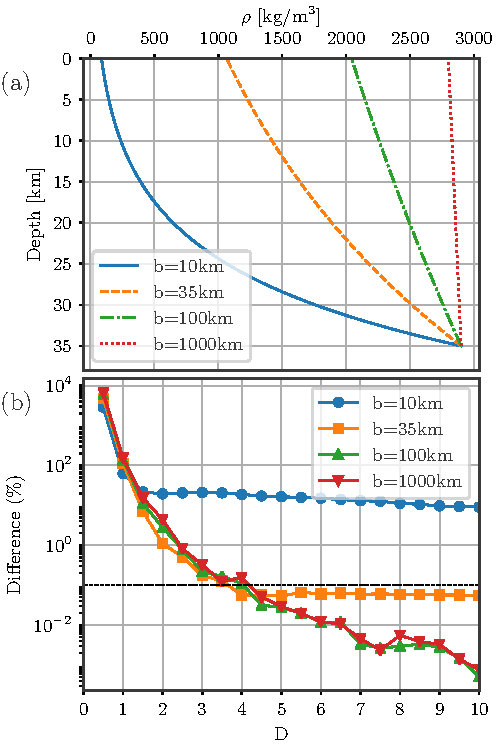
\includegraphics[width=0.9\linewidth]{figures/Dexp-power-differences-thick.pdf}
\caption{
    Results of the accuracy tests for different exponential density functions in case of a thick spherical shell (35km of thickness).
    (a) Density functions used in the tests, each one with a different value of $b$ and normalised in such way that they reaches a density of 2900kg/m$^{3}$ at the bottom of the shell.
    (b) Differences between the Marussi tensor component $g_{zz}$ generated by the numerical model and the analytical solution for each density function. Each computation was performed on the big grid described in Table \ref{tab:grids}, for different values of the distance-size ratio $D$. If the difference is less than 0.1\%, we consider that the model has achieved an acceptable accuracy for the corresponding value of $D$.
}
\label{fig:D-exp-power-thick}
\end{figure}


\subsection{Discontinuous Density}

As a final case, we performed the same test with a discontinuous density function:

\begin{equation}
    \rho(r') = 
    \begin{cases}
        \rho_1 & \text{if} \, R_1 \leq r' < R_c \\
        \rho_2 & \text{if} \, R_c \leq r' \leq R_2 \\
    \end{cases}
\label{eq:density-discontinuous}
\end{equation}

\noindent where $\rho_1$ and $\rho_2$ are constant densities, $R_1$ and $R_2$ are the inner and outer radii of the shell, respectively, and $R_c$ is the the radius on which the 
density changes.

The analytical solution for this kind of density is the linear combination of two homogeneous shells with densities $\rho_1$ and $\rho_2$:

\begin{equation}
    V(r) = \frac{4}{3} \frac{\pi G}{r}
    \left[ \rho_1 (R_c^3 - R_1^3) +
    \rho_2 (R_2^3 - R_c^3) \right]
\end{equation}

Firstly, lets assume a symmetric density function, i.e. $R_c=(R_1 + R_2)/2$ is the centre radius of the shell, and perform the test for a thin shell of 1km of thickness.
The results can be seen in Figure \ref{fig:D-discont-sym}.
Again, we obtain good accuracy for values of $D$ equal to 1, 2 and 8 for the computation of the potential, the gradient components and the Marussi tensor components, respectively.

\begin{figure}
\centering
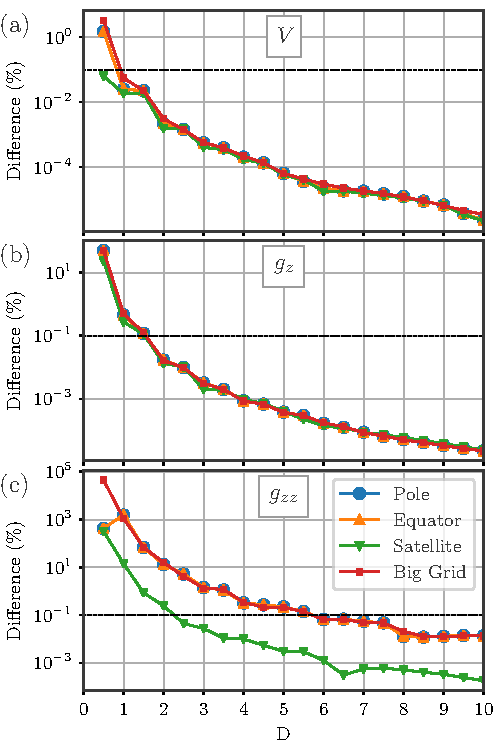
\includegraphics[width=0.9\linewidth]{figures/Ddiscontinuous-symmetric-differences.pdf}
\caption{
    Differences between the gravity fields generated by the numerical model and the analytical solution for a thin spherical shell of 1km of thickness with the discontinuous density defined on equation \ref{eq:density-discontinuous} and $R_c$ as the centre radius of the shell. The computations were performed on the four grids described in Table \ref{tab:grids} and for different values of the distance-size ratio $D$. If the difference is less than 0.1\%, we consider that the model has achieved an acceptable accuracy for the corresponding value of $D$.
}
\label{fig:D-discont-sym}
\end{figure}

Secondly, lets assume the same density function from equation \ref{eq:density-discontinuous}, but now with an asymmetrical distribution: $R_c = (R_1 + R_2)/3$, and perform the same test.
We can see its results in Figure \ref{fig:D-discont-asym}: up to $D=10$ the difference between the numerical model and the analytical solution is greater than 10\%, what
leads us to conclude that the code does not recreates the gravity fields for this case with good accuracy.

\begin{figure}
\centering
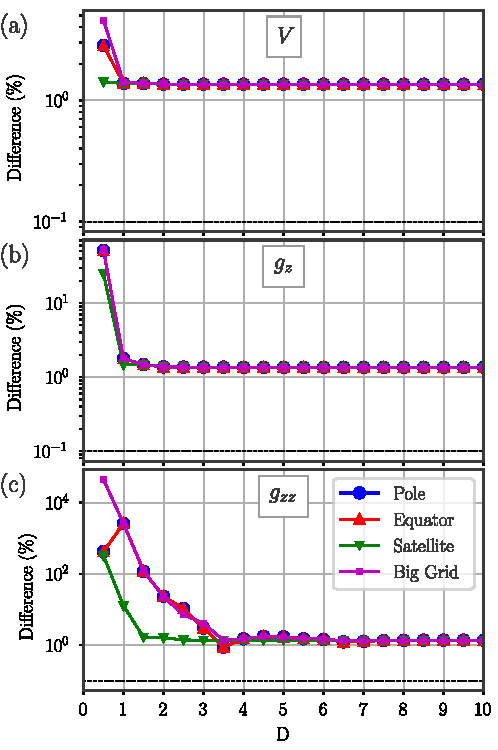
\includegraphics[width=0.9\linewidth]{figures/Ddiscontinuous-asymmetric-differences.pdf}
\caption{
    Differences between the gravity fields generated by the numerical model and the analytical solution for a thin spherical shell of 1km of thickness with the discontinuous density defined on equation \ref{eq:density-discontinuous} and $R_c=(R_1 + R_2)/3$. The computations were performed on the four grids described in Table \ref{tab:grids} and for different values of the distance-size ratio $D$. If the difference is less than 0.1\%, we consider that the model has achieved an acceptable accuracy for the corresponding value of $D$.
}
\label{fig:D-discont-asym}
\end{figure}

From equation \ref{eq:glq-var-dens} we have seen that the information of the density function is summarised as the values its assumes on the nodes of the GLQ.
We can attribute the low performance of the code to this simplification.

On the other hand, we can explain the good performance in the symmetrical density case due to the fact that the GLQ nodes are always symmetrical with respect to the centre of the $[a,b]$ integration interval (see equation \ref{eq:glq-scaled}).

In the light of these results we do not recommend using discontinuous densities functions. Instead, divide the tesseroid into several ones with specific homogeneous density or density function for each one.


%%%%%%%%%%%%%%%%%%%%%%%%%%%%%%%%%%%%%%%%%%%%%%%%%%%%%%%%%%%%%%%%%%%%%%%%%%%%%%%

\section{Speed Comparison}

We have recorded the computation times for the gravity potential, the gradient component $g_z$ and the Marussi tensor component $g_{zz}$ generated by a single tesseroid model with homogeneous ($\Delta t_\text{homogeneous}$) and variable ($\Delta 
t_\text{variable}$) density at different heights. Then we plotted the ratio between these computation times (see Figure \ref{fig:speed-comparison}): 

\begin{equation}
    \text{Computation Times Ratio} =
        \frac{\Delta t_\text{variable}}{\Delta t_\text{homogeneous}}
    \label{eq:computation-times-ratio}
\end{equation}

From these results we can conclude that the homogeneous density code is up to twice faster than the new variable density algorithm for lower heights. However, the computation times ratio gets lower at greater heights, due to the reduction of the divisions made by the adaptive discretization algorithm. In summary, the new variable density code is fast enough to perform the calculations of a real model in a few minutes. \todo{real, esta bien la expresion?}

\begin{figure}
\centering
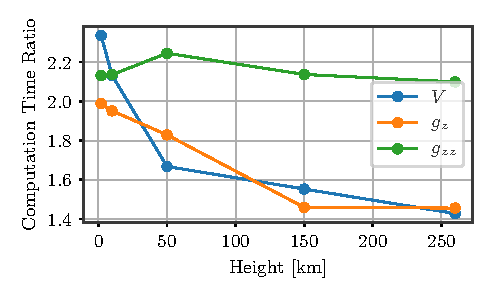
\includegraphics[width=0.9\linewidth]{figures/speed-comparison.pdf}
\caption{Computation times ratio between a single tesseroid model with variable and with homogeneous density at different heights, defined in equation \ref{eq:computation-times-ratio}.}
\label{fig:speed-comparison}
\end{figure}


%%%%%%%%%%%%%%%%%%%%%%%%%%%%%%%%%%%%%%%%%%%%%%%%%%%%%%%%%%%%%%%%%%%%%%%%%%%%%%%

\section{Conclusions}

We have developed a Python library that allows us to perform forward gravity computations using tesseroids with variable density in depth.
The code numerically approximates the integral that defines the gravity potential, its gradient and the Marussi tensor through the Gauss-Legendre Quadrature (GLQ).
It essentially consists in approximating the gravity fields of the tesseroids with the effect of point masses located on the scaled nodes of the Legendre polynomials.
We have stated that this method it's well suited to approximate the effect of tesseroids with arbitrary densities, in contrast with the ones that involve Taylor series expansion.

Instead of enhancing the accuracy of the method by increasing the order of the GLQ on each integration, we make use of the modified adaptive discretization algorithm.
It divides the tesseroid by half if the ratio of the distance to the computation point and its size is lower than a predefined distance-size ratio $D$.
We can summarise that $D$ controls the accuracy of the method: a higher value of $D$ generates more divisions of the tesseroids, thus more point masses, what leads to a more precise approximation.

On the other hand, there's no direct relation between the value of $D$ and the error of the computation, that's why we had to determine the minimum value of $D$ that produces an acceptable accuracy for each gravity magnitude.
These distance-size ratio determinations have been made through the comparison of the numerical approximation with the analytical solutions for the exceptional case of a spherical shell.
From the wide range of possible density variations, we've chosen a linear, an exponential and a discontinuous density functions.

The tests over the first two functions have shown that in order to achieve an accuracy of 0.1\%, a value of $D$ equal to 1, 2 and 8 must be used in the calculation of the gravity potential, its gradient components and the components of the Marussi tensor, respectively.
We have also found a limitation on the variation of the exponential density function: the absolute value of the exponent must not be greater than 1.
However, those extremely variations cannot be found inside the Earth, so this limitation does not determines a true restriction for real life models.

On the other hand, the tests over the discontinuous function were not satisfactory.
In such cases we recommend to divide the model in several tesseroids, each one with a specific homogeneous density or a continuous density function, instead of using a single variable density tesseroid.

%%%%%%%%%%%%%%%%%%%%%%%%%%%%%%%%%%%%%%%%%%%%%%%%%%%%%%%%%%%%%%%%%%%%%%%%%%%%%%%

\section{Acknowledgments}

We are indebted to the developers and maintainers of the open-source
software without which this work would not have been possible.

%%%%%%%%%%%%%%%%%%%%%%%%%%%%%%%%%%%%%%%%%%%%%%%%%%%%%%%%%%%%%%%%%%%%%%%%%%%%%%%

\bibliographystyle{gji}
\bibliography{bibtex/references}

\end{document}
